% \appendix\label{appendix:2d_old}
% \appendixpage
% \addappheadtotoc

\begin{appendices}
\chapter*{Appendice}\label{appendix}
\section*{Grafici omessi nel~\Cref{chap:esperimenti}}
\begin{figure}[!ht]
    \begin{subfigure}{.4999\textwidth}
        \centering
        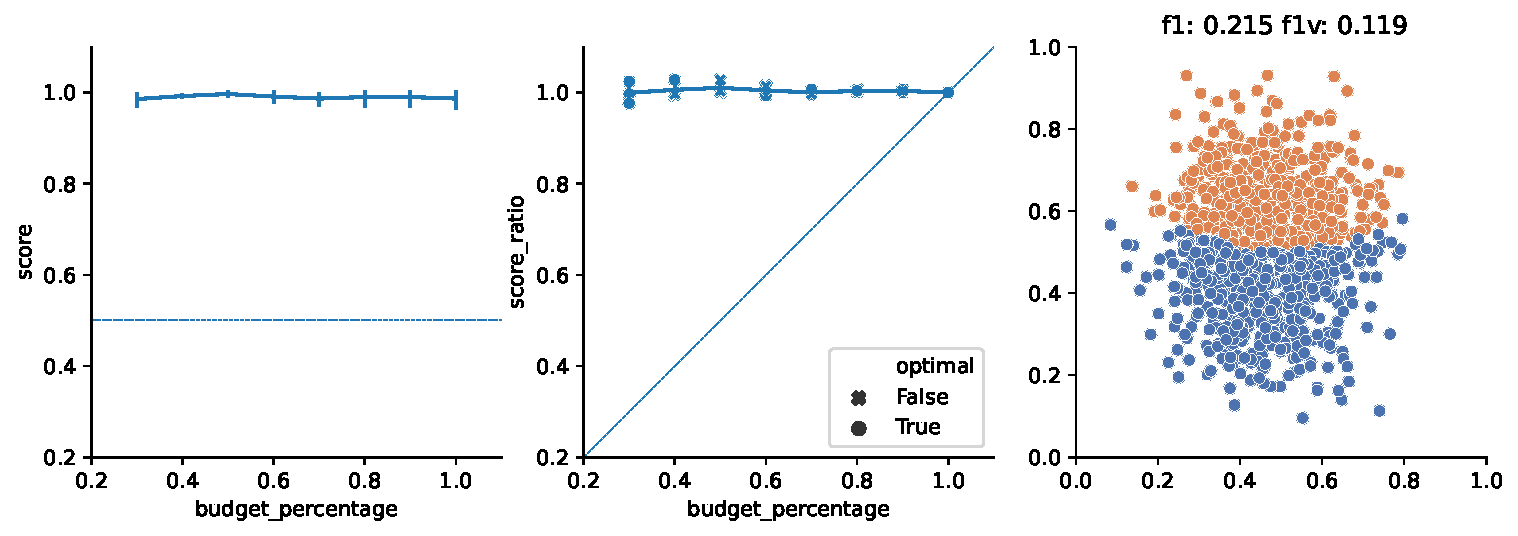
\includegraphics[width=\textwidth]{img/2d/1.pdf}
    \end{subfigure}%
    \begin{subfigure}{.5\textwidth}
        \centering
        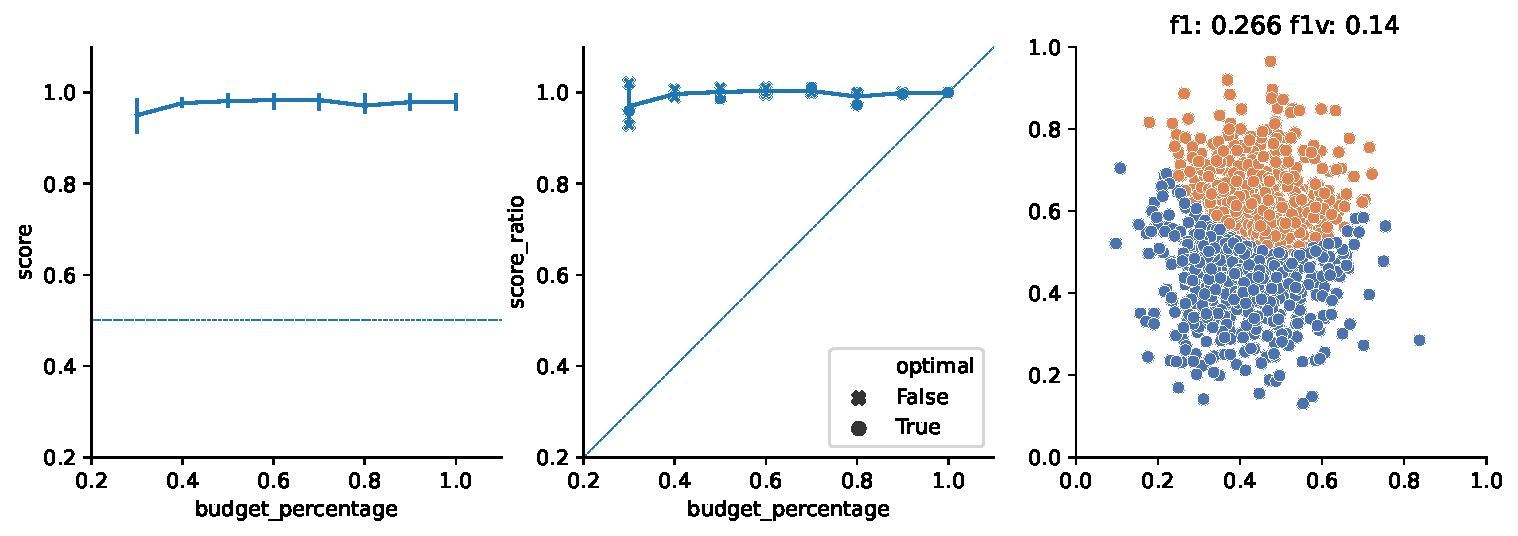
\includegraphics[width=\textwidth]{img/2d/2.pdf}
    \end{subfigure}%
    %
    \hfill
    %
    \begin{subfigure}{.5\textwidth}
        \centering
        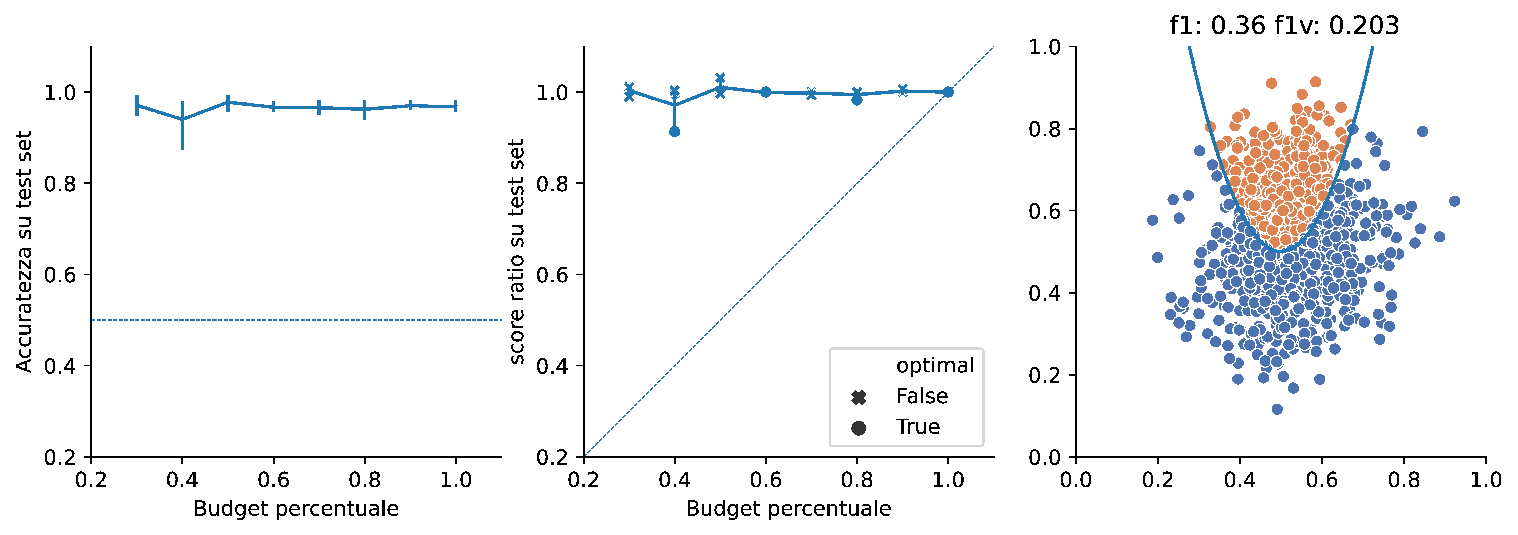
\includegraphics[width=\textwidth]{img/2d/5.pdf}
    \end{subfigure}%
    \begin{subfigure}{.5\textwidth}
        \centering
        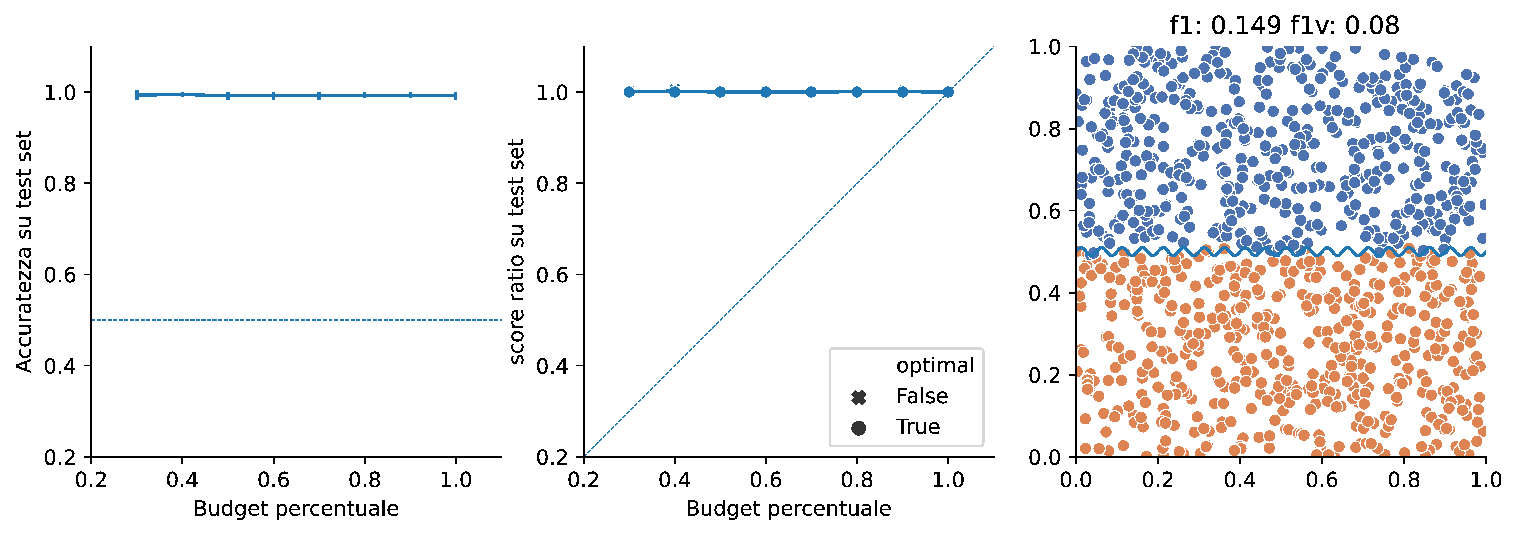
\includegraphics[width=\textwidth]{img/2d/6.pdf}
    \end{subfigure}%
    %
    \hfill
    %
    \begin{subfigure}{.5\textwidth}
        \centering
        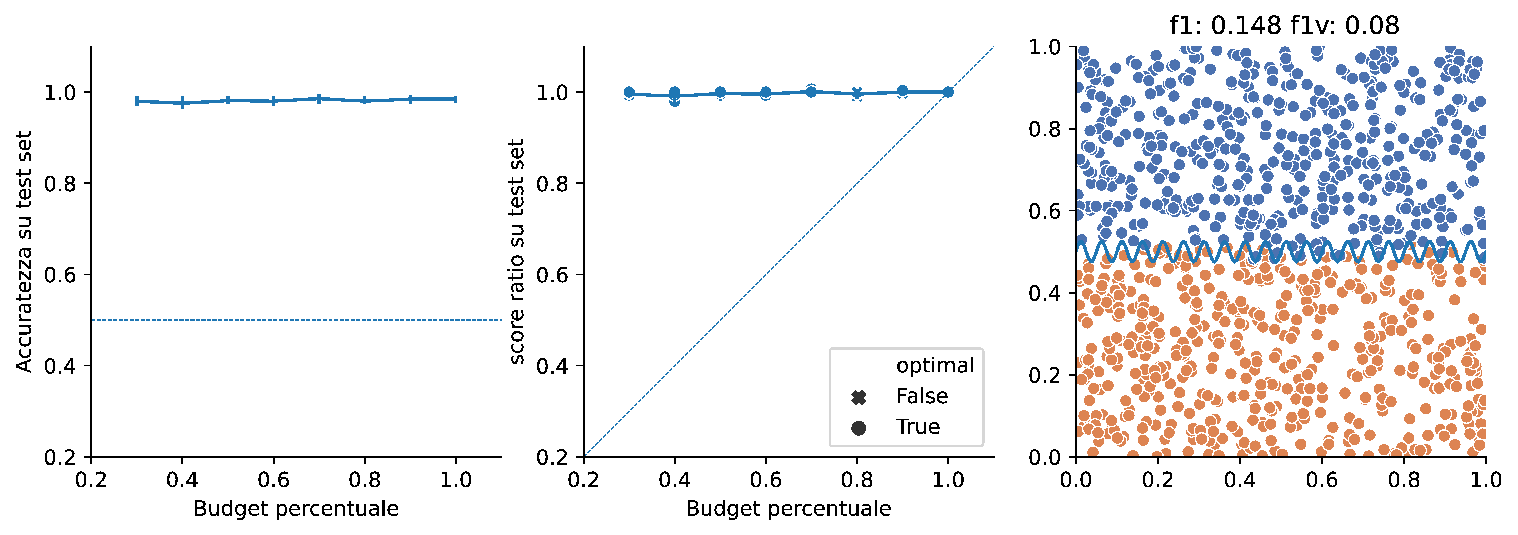
\includegraphics[width=\textwidth]{img/2d/7.pdf}
    \end{subfigure}%
    \begin{subfigure}{.5\textwidth}
        \centering
        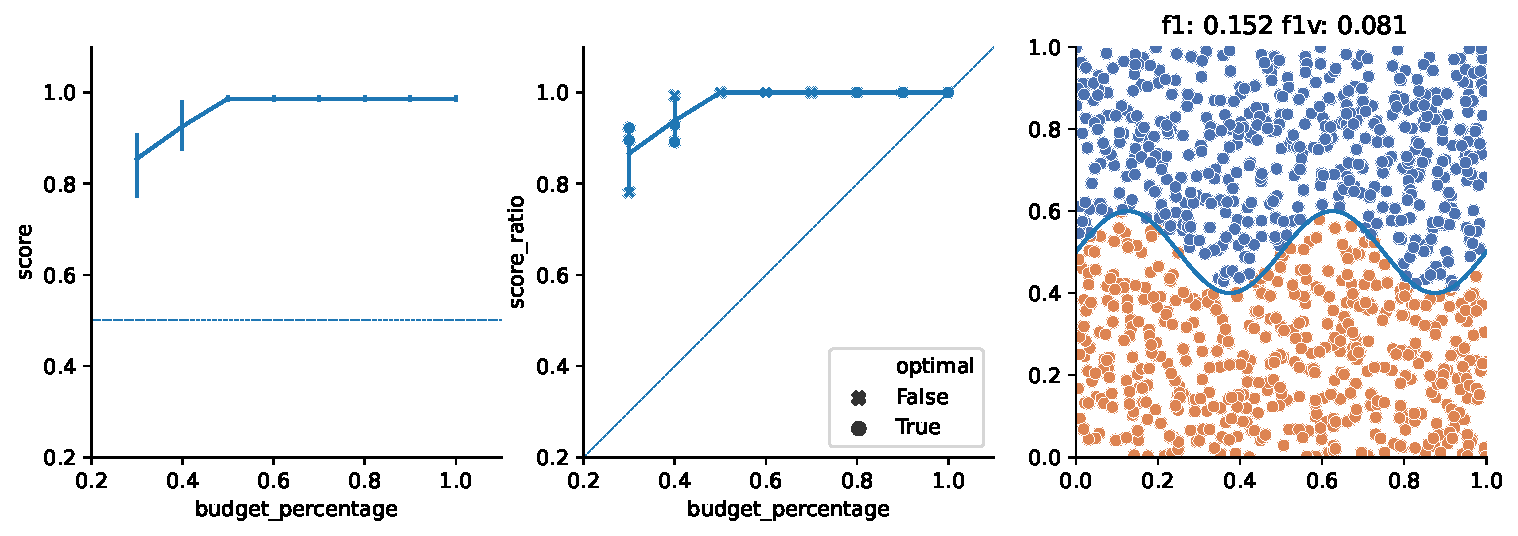
\includegraphics[width=\textwidth]{img/2d/11.pdf}
    \end{subfigure}%
    \caption{Questi grafici completano la~\Cref{fig:risultati_2d}.}
\end{figure}

\begin{figure}
    \begin{subfigure}{.5\textwidth}
        \centering
        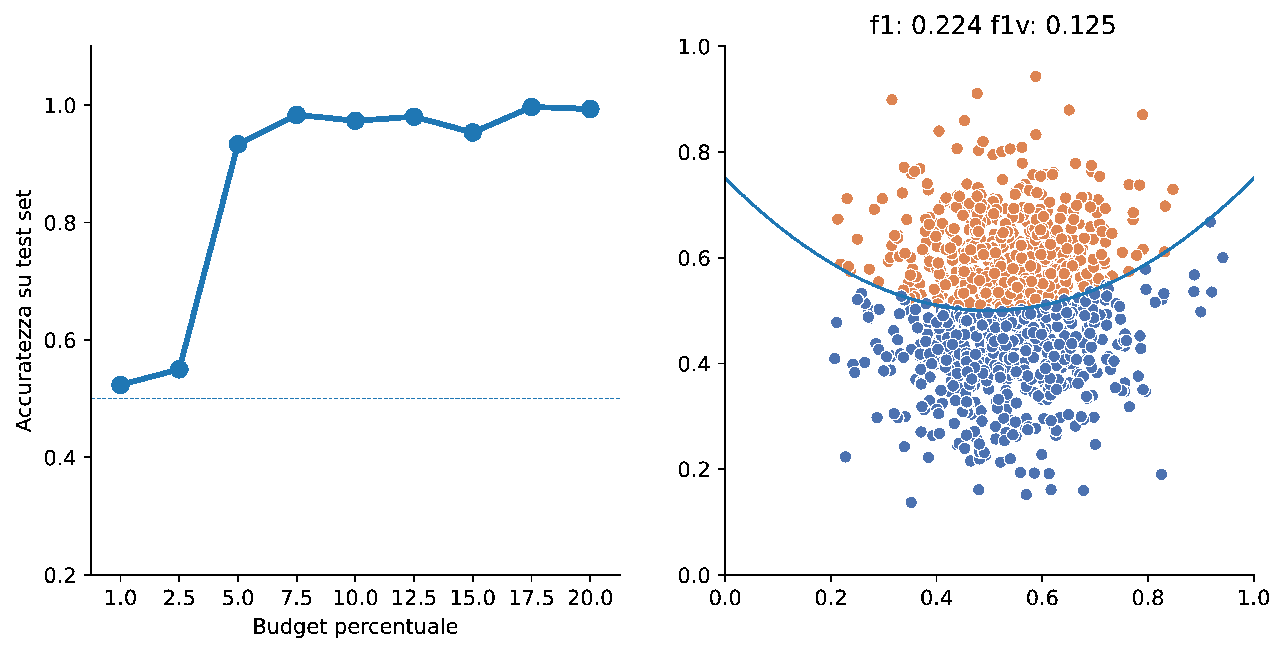
\includegraphics[width=\textwidth]{img/2d_v2/1.pdf}
    \end{subfigure}%
    \begin{subfigure}{.5\textwidth}
        \centering
        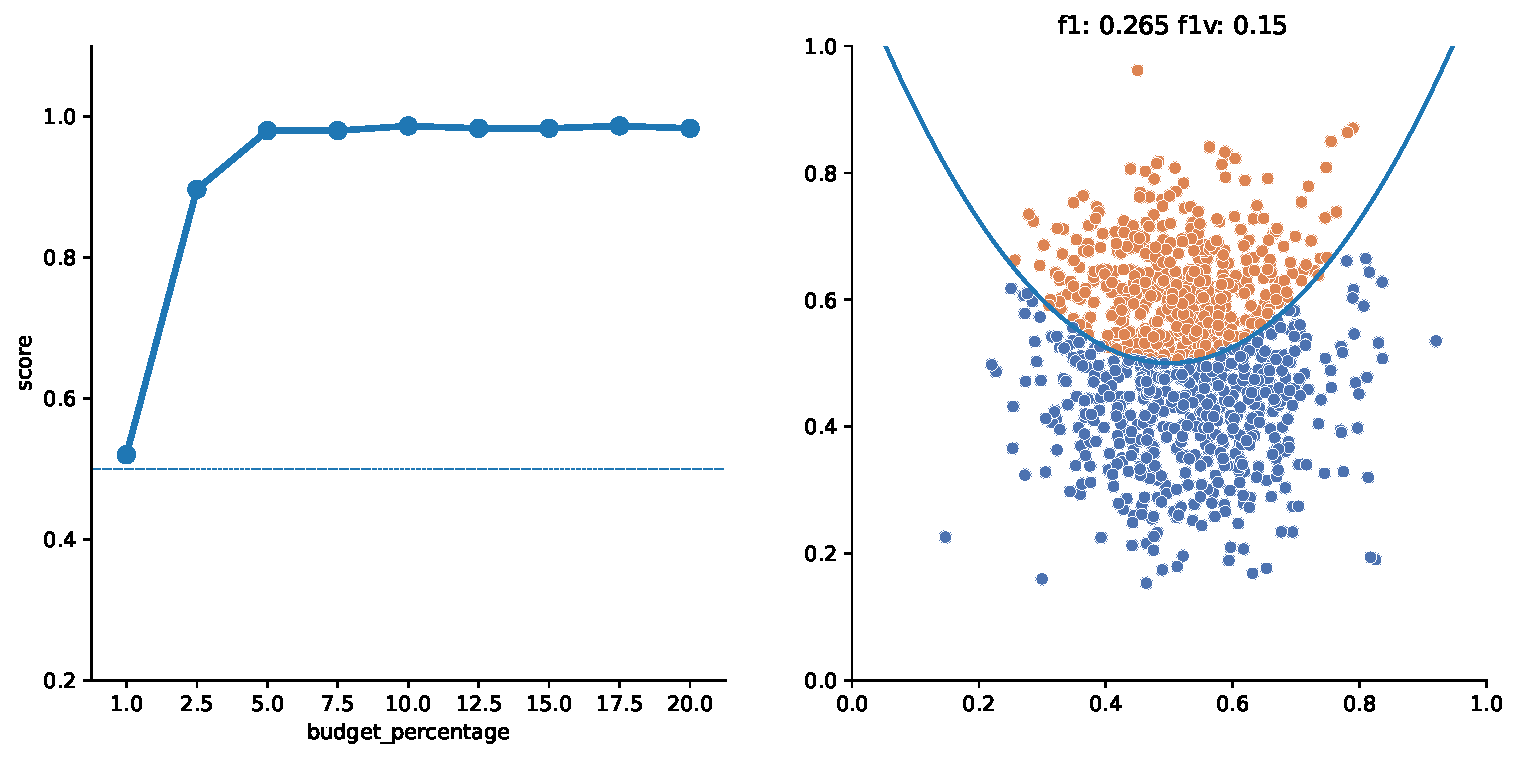
\includegraphics[width=\textwidth]{img/2d_v2/2.pdf}
    \end{subfigure}
    %
    \hfill
    %
    \begin{subfigure}{.5\textwidth}
        \centering
        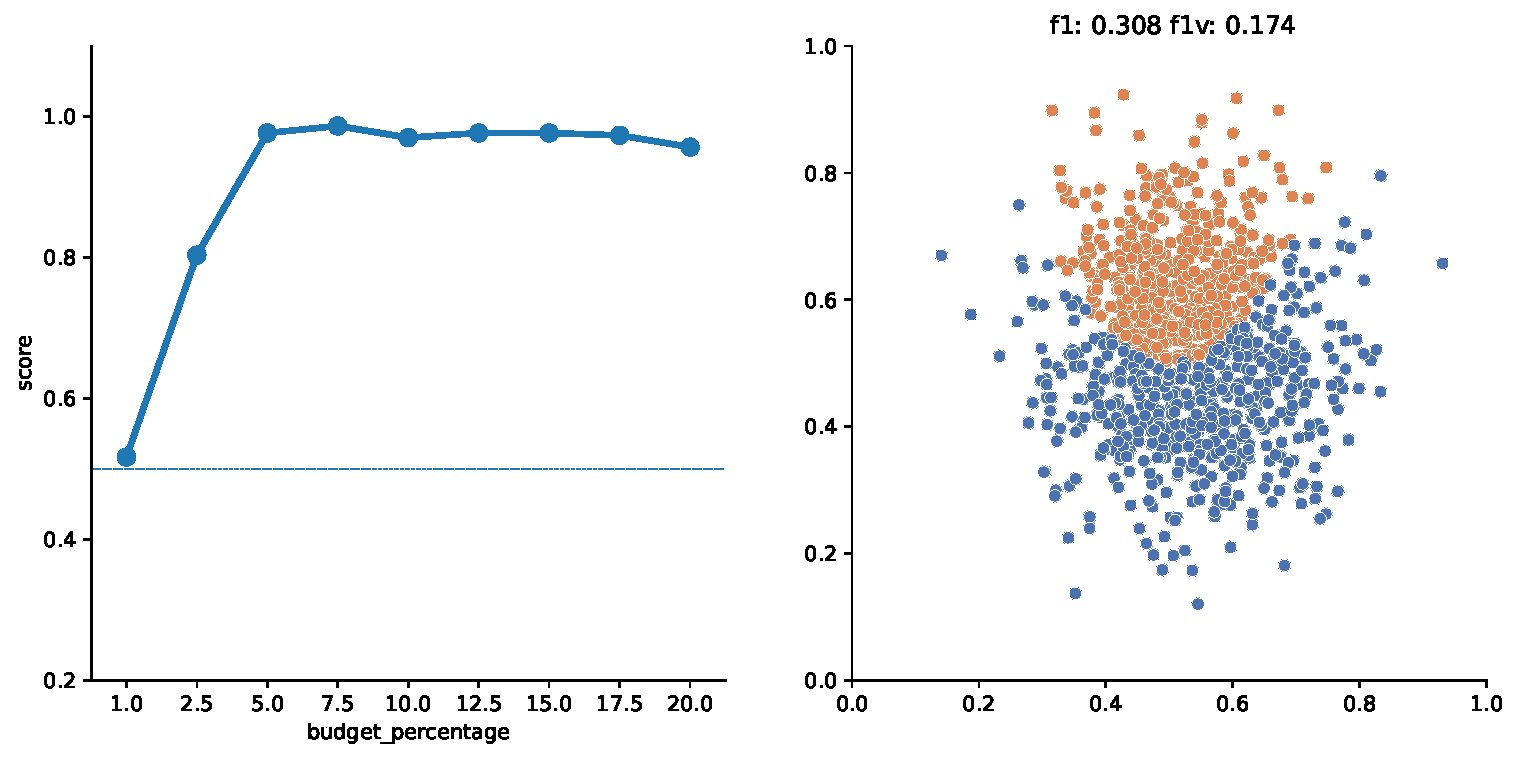
\includegraphics[width=\textwidth]{img/2d_v2/3.pdf}
    \end{subfigure}
    \begin{subfigure}{.5\textwidth}
        \centering
        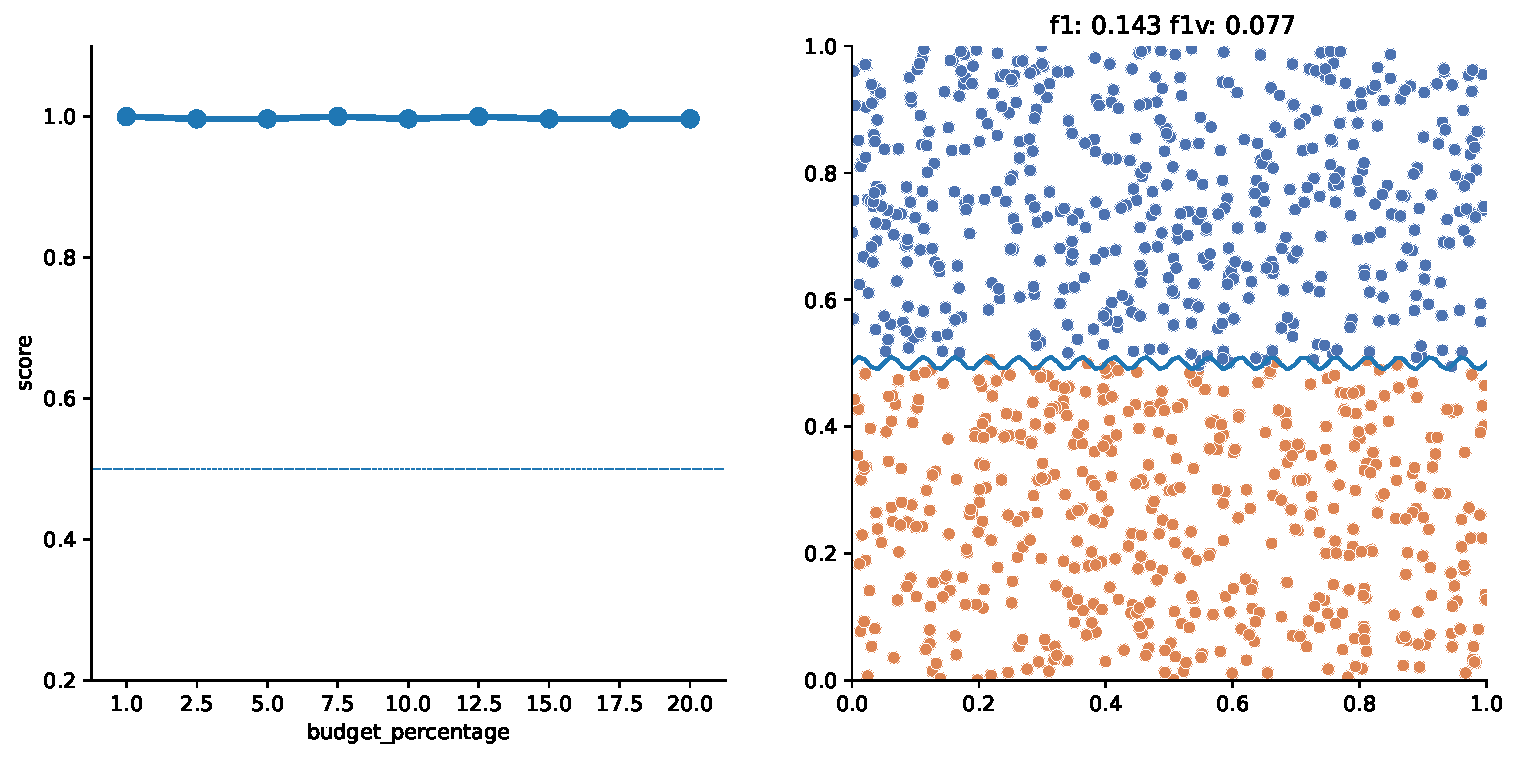
\includegraphics[width=\textwidth]{img/2d_v2/6.pdf}
    \end{subfigure}%
    %
    \hfill
    %
    \begin{subfigure}{.5\textwidth}
        \centering
        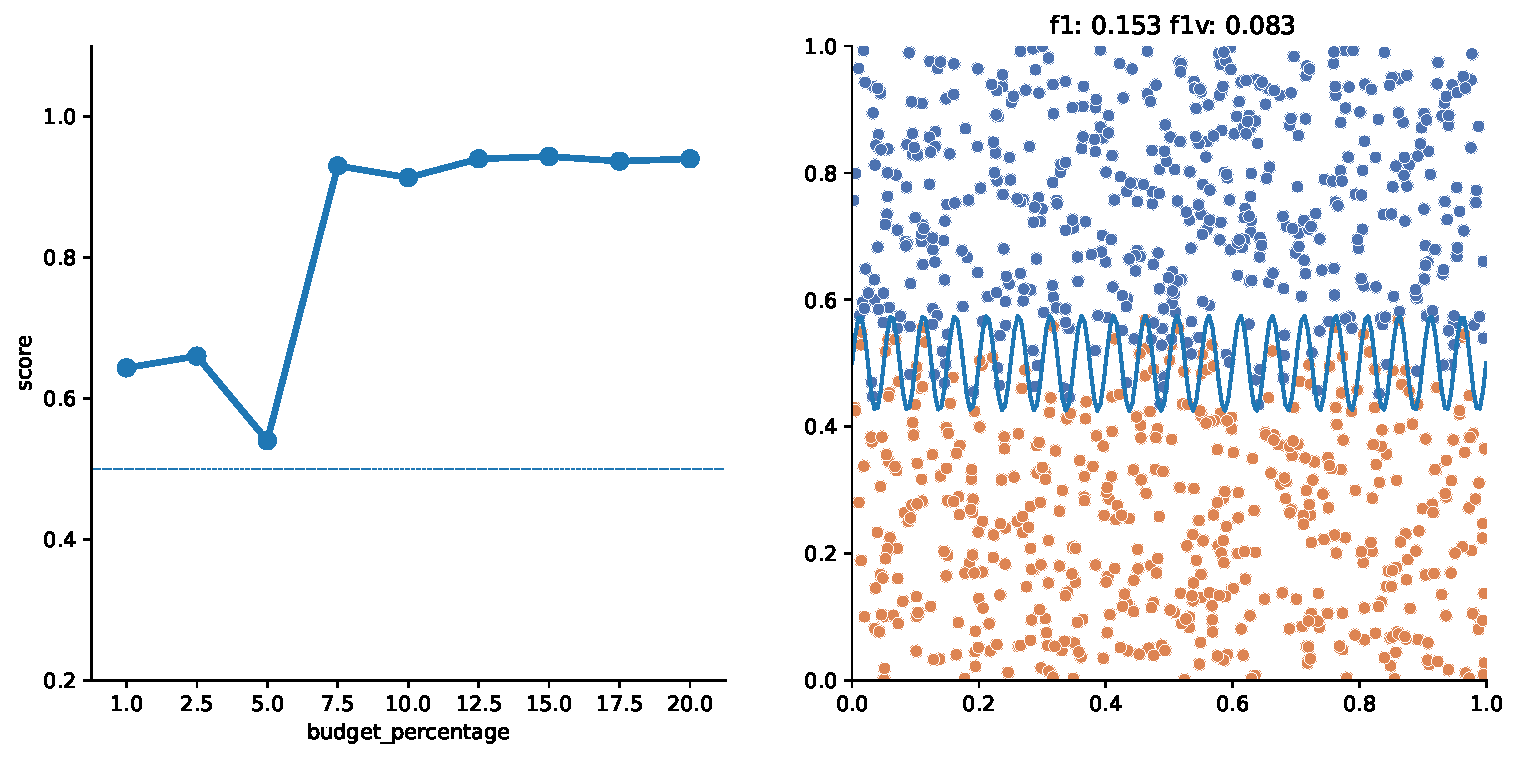
\includegraphics[width=\textwidth]{img/2d_v2/9.pdf}
    \end{subfigure}
    \begin{subfigure}{.5\textwidth}
        \centering
        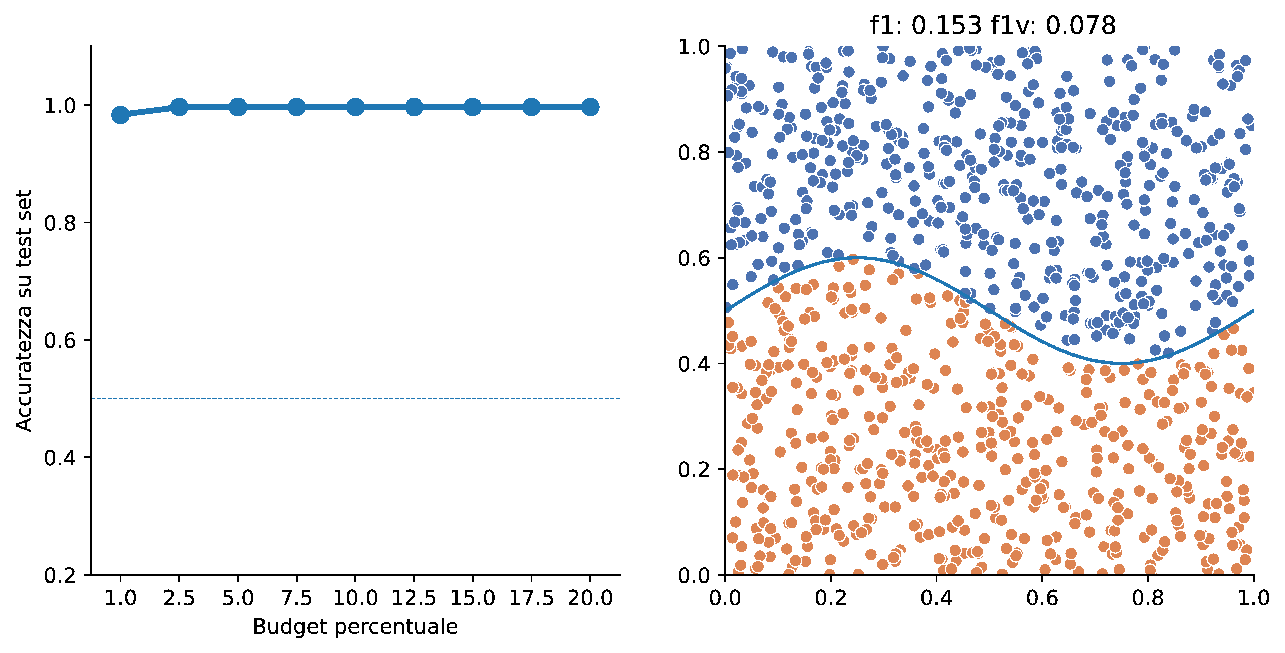
\includegraphics[width=\textwidth]{img/2d_v2/10.pdf}
    \end{subfigure}%
    %
    \hfill
    %
    \begin{subfigure}{.5\textwidth}
        \centering
        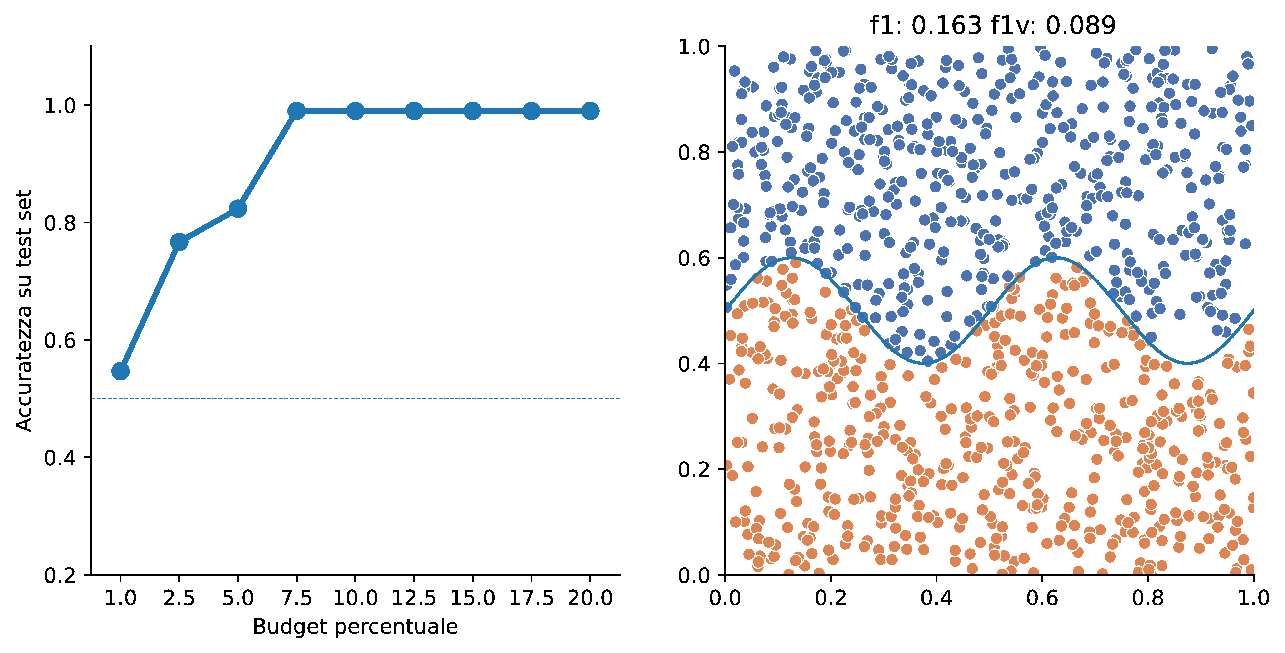
\includegraphics[width=\textwidth]{img/2d_v2/11.pdf}
    \end{subfigure}
\caption{Questi grafici completano la~\Cref{fig:2d_v2}.}
\end{figure}

\begin{figure}
    \begin{subfigure}{.5\textwidth}
        \centering
        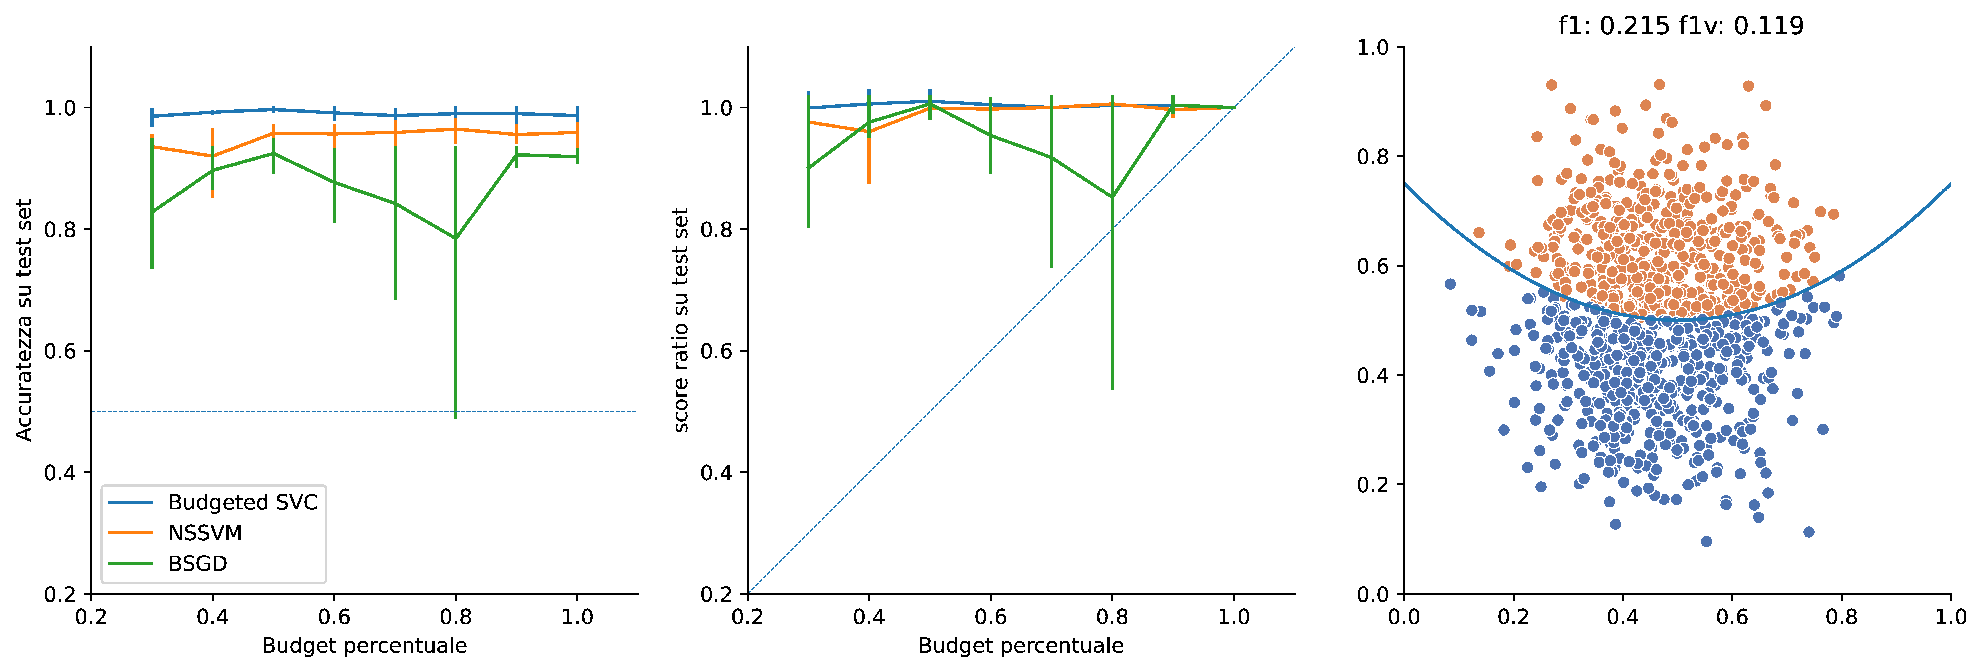
\includegraphics[width=\textwidth]{img/comp_old/1.pdf}
    \end{subfigure}%
    \begin{subfigure}{.5\textwidth}
        \centering
        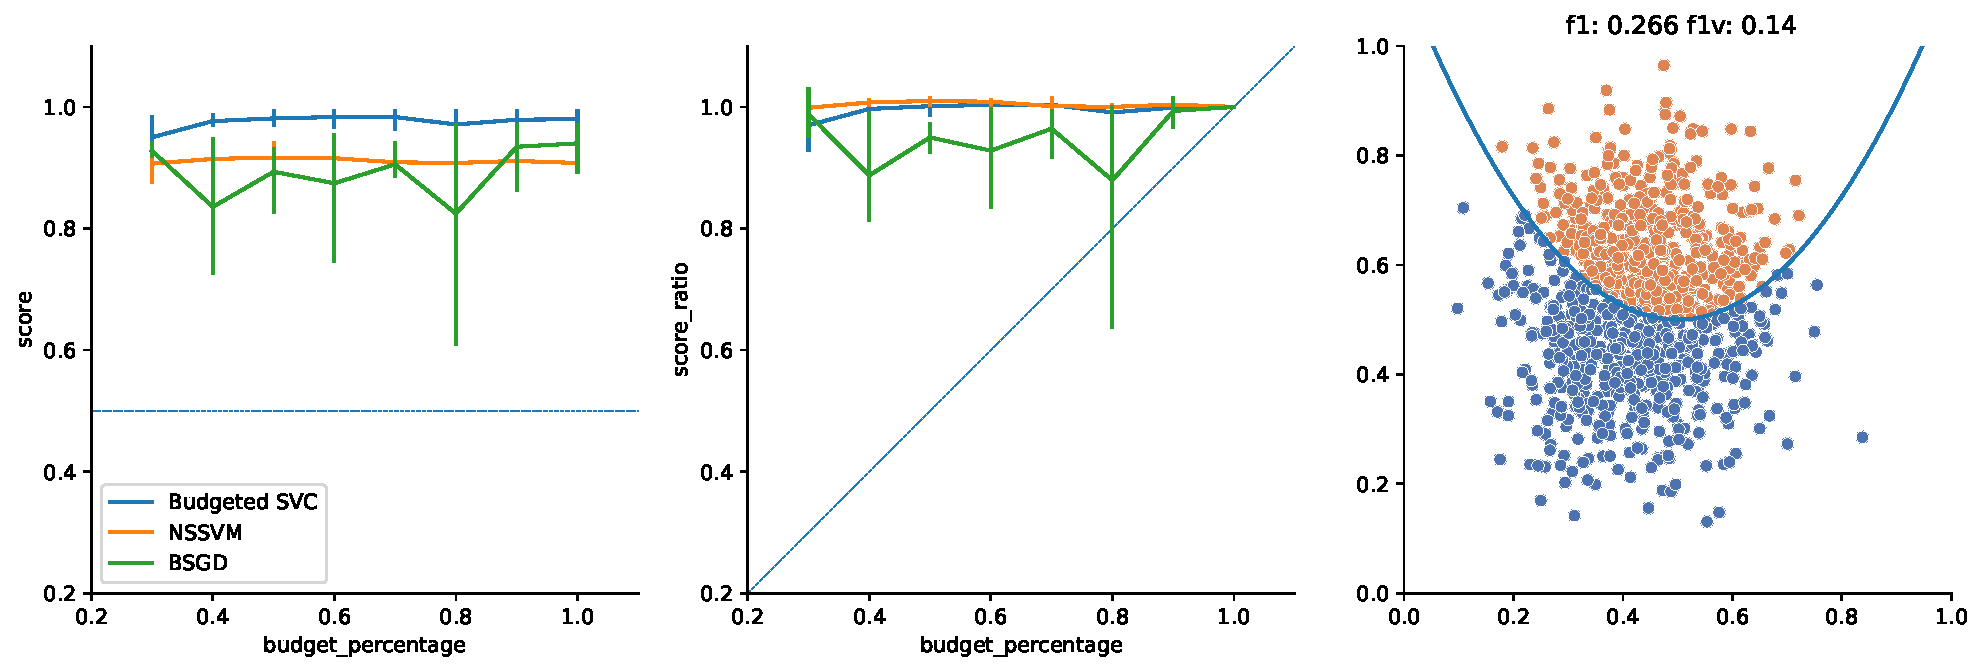
\includegraphics[width=\textwidth]{img/comp_old/2.pdf}
    \end{subfigure}
    %
    \hfill
    %
    \begin{subfigure}{.5\textwidth}
        \centering
        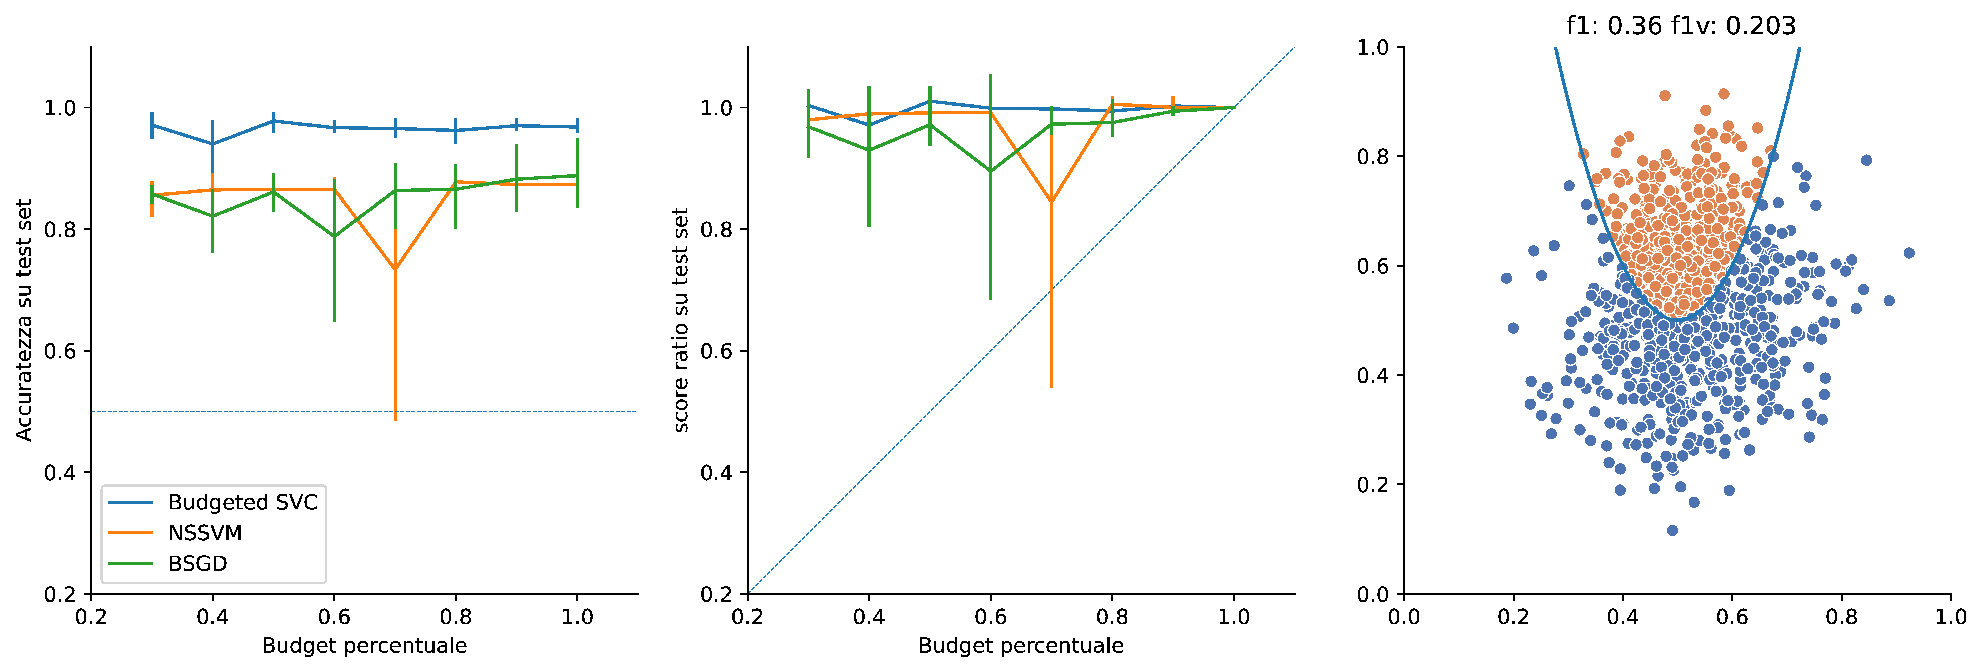
\includegraphics[width=\textwidth]{img/comp_old/5.pdf}
    \end{subfigure}
    \begin{subfigure}{.5\textwidth}
        \centering
        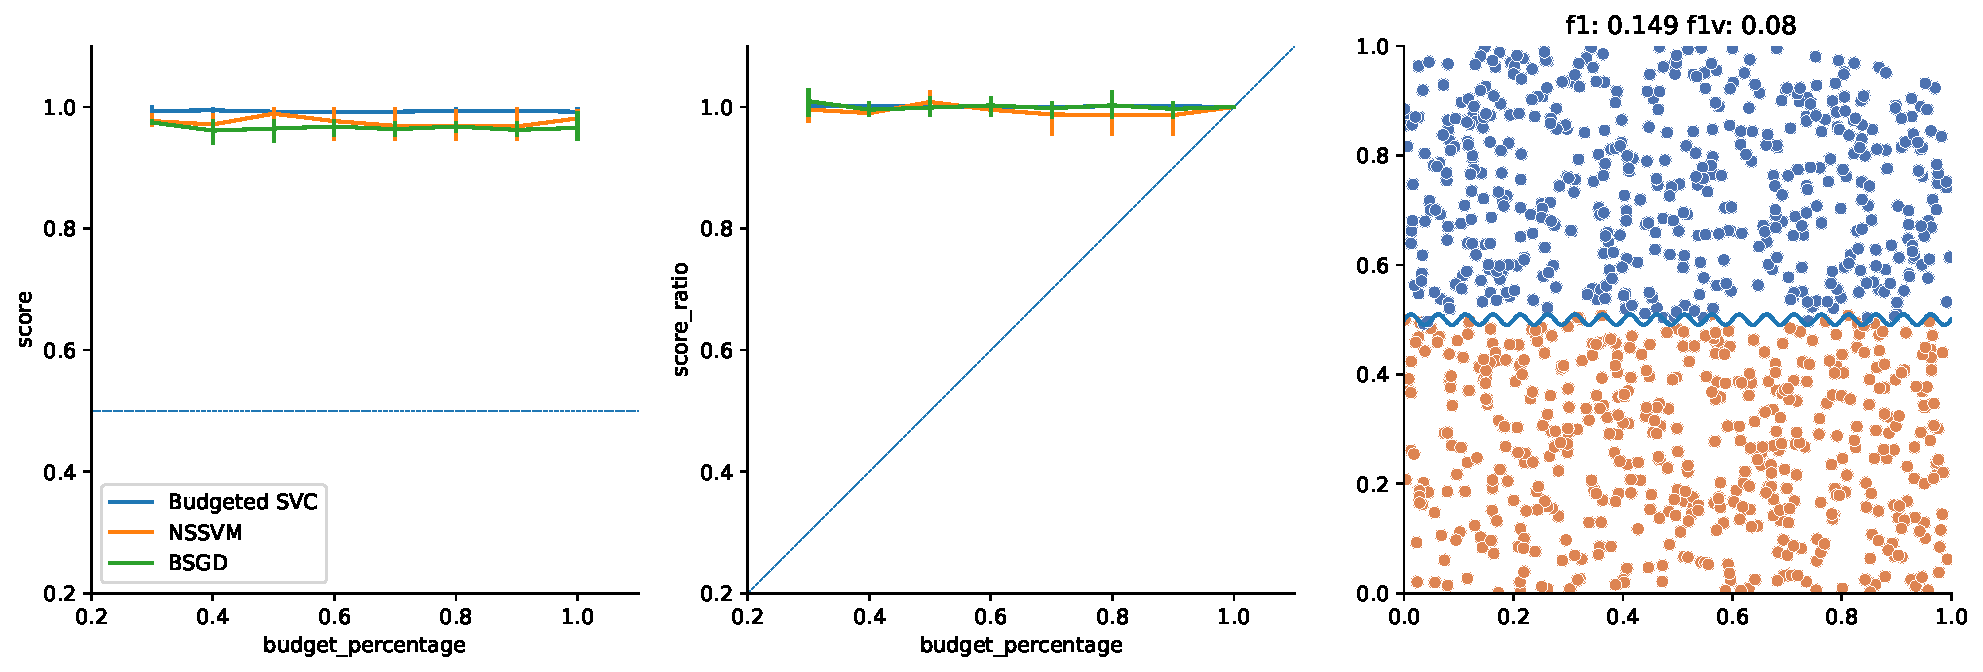
\includegraphics[width=\textwidth]{img/comp_old/6.pdf}
    \end{subfigure}%
    %
    \hfill
    %
    \begin{subfigure}{.5\textwidth}
        \centering
        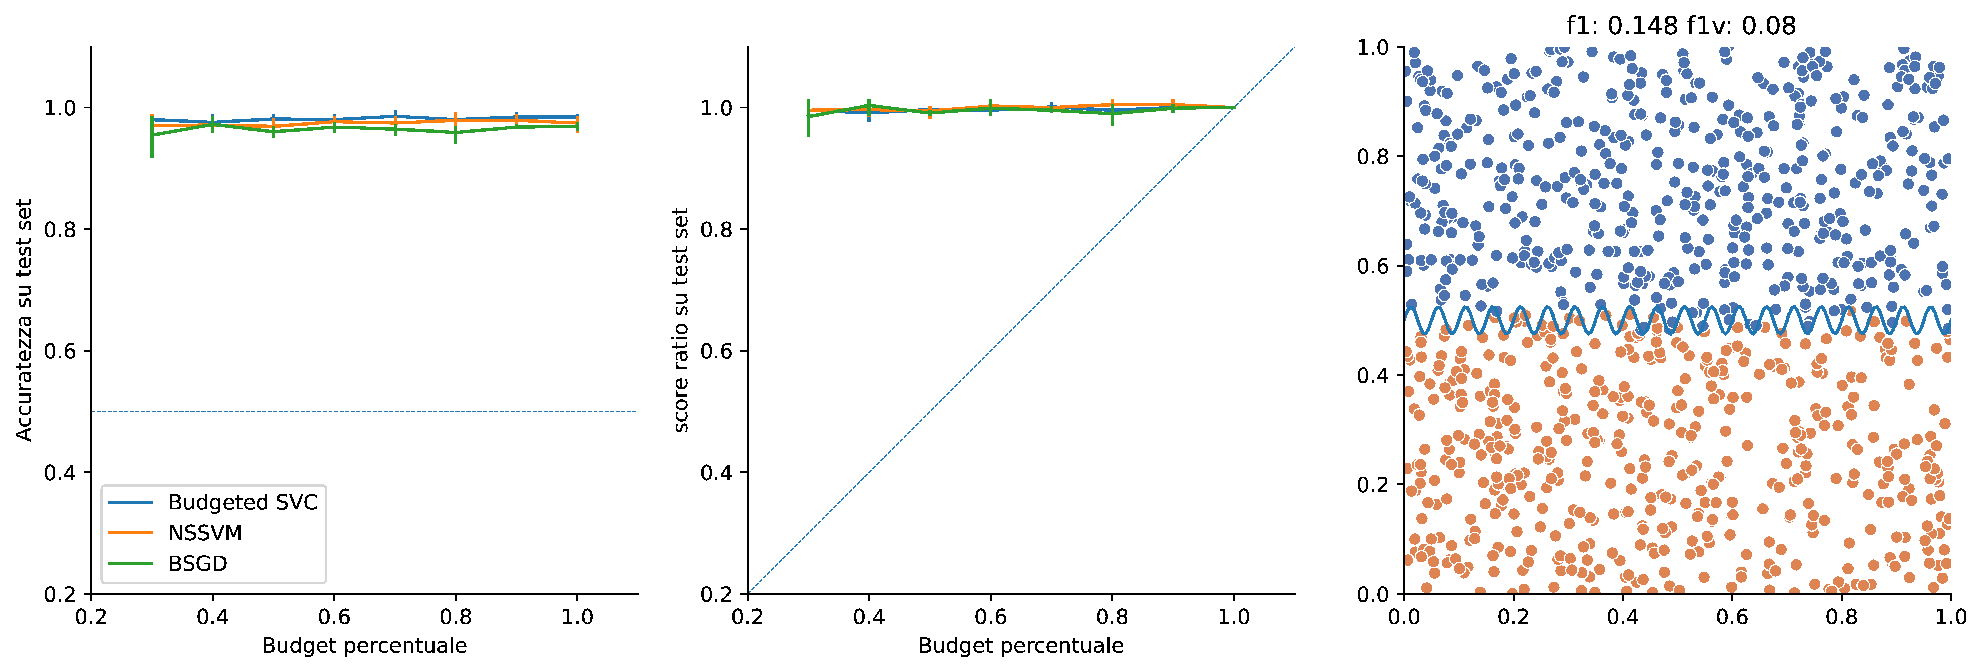
\includegraphics[width=\textwidth]{img/comp_old/7.pdf}
    \end{subfigure}
    \begin{subfigure}{.5\textwidth}
        \centering
        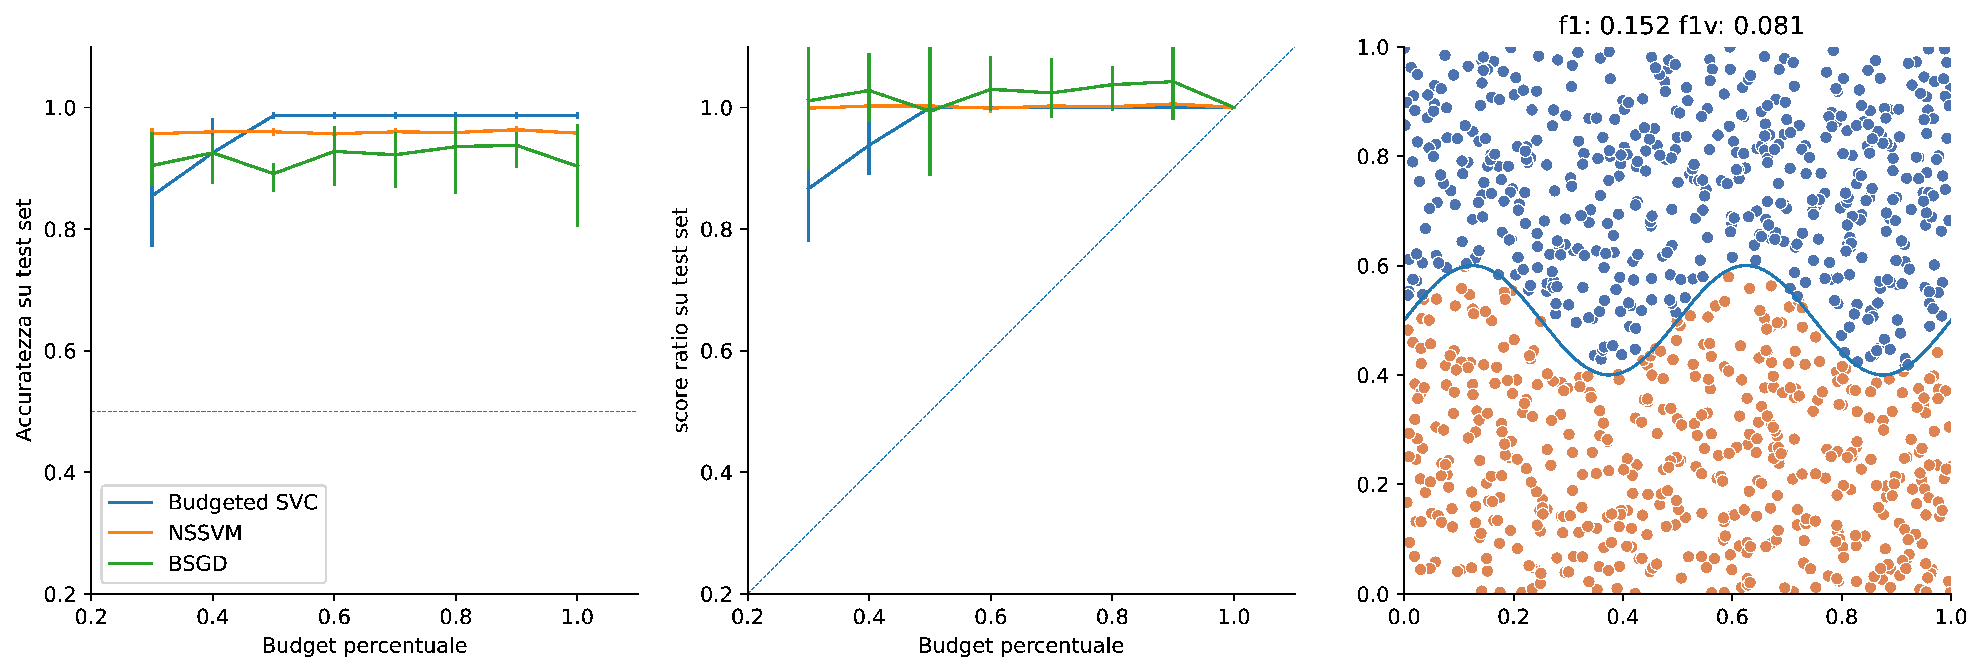
\includegraphics[width=\textwidth]{img/comp_old/11.pdf}
    \end{subfigure}%
\caption{Questi grafici completano la~\Cref{fig:comp_old}.}
\end{figure}

\begin{figure}
    \begin{subfigure}{.5\textwidth}
        \centering
        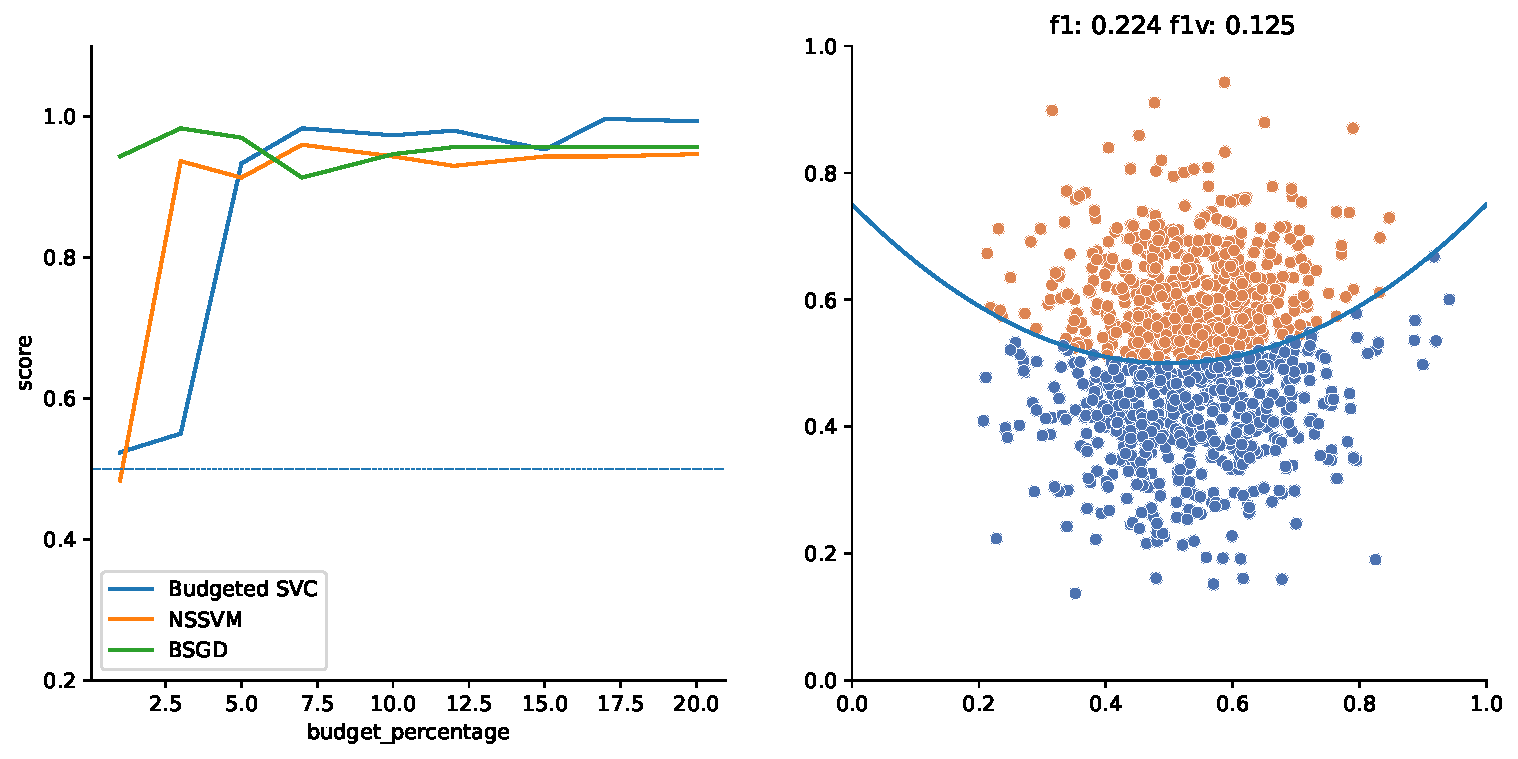
\includegraphics[width=\textwidth]{img/comp_new/1.pdf}
    \end{subfigure}%
    \begin{subfigure}{.5\textwidth}
        \centering
        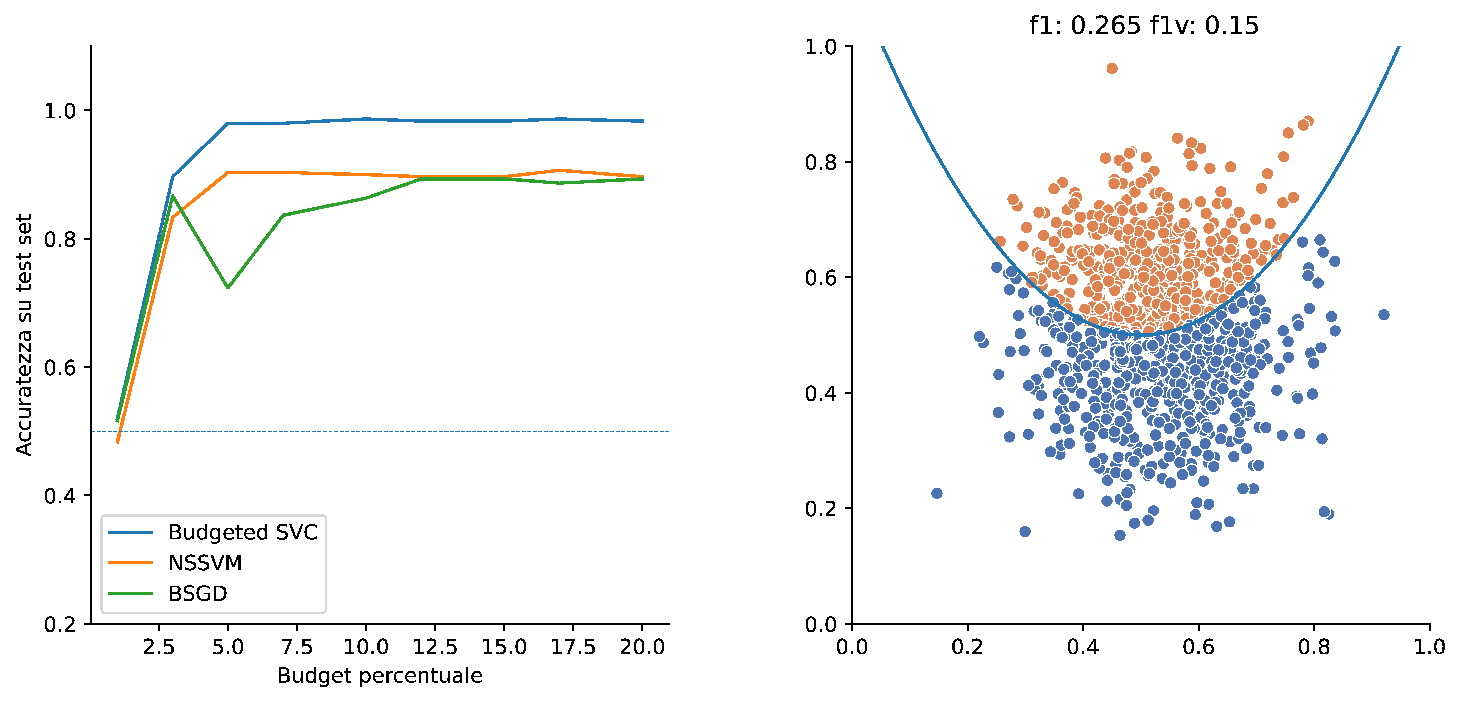
\includegraphics[width=\textwidth]{img/comp_new/2.pdf}
    \end{subfigure}
    %
    \hfill
    %
    \begin{subfigure}{.5\textwidth}
        \centering
        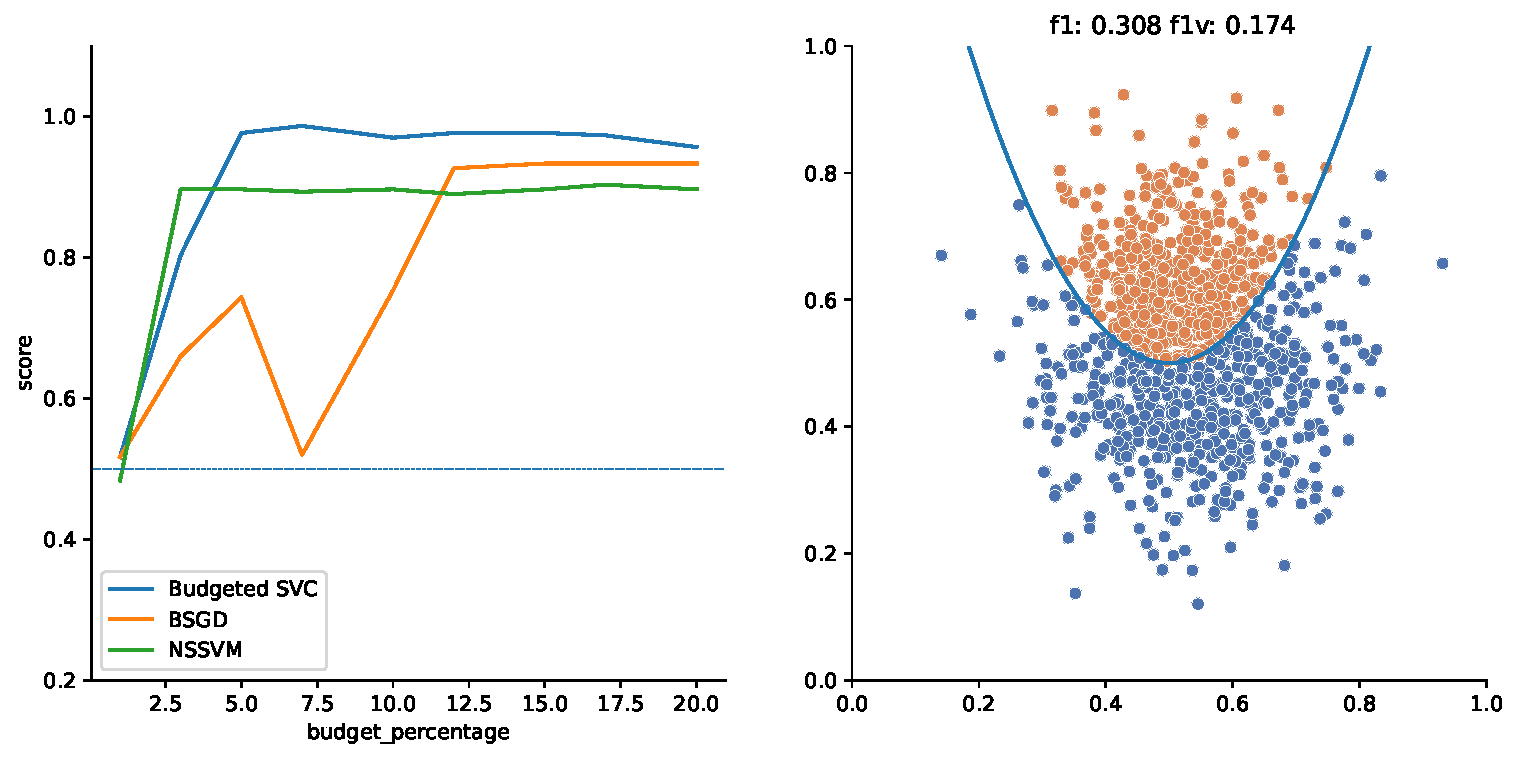
\includegraphics[width=\textwidth]{img/comp_new/3.pdf}
    \end{subfigure}
    \begin{subfigure}{.5\textwidth}
        \centering
        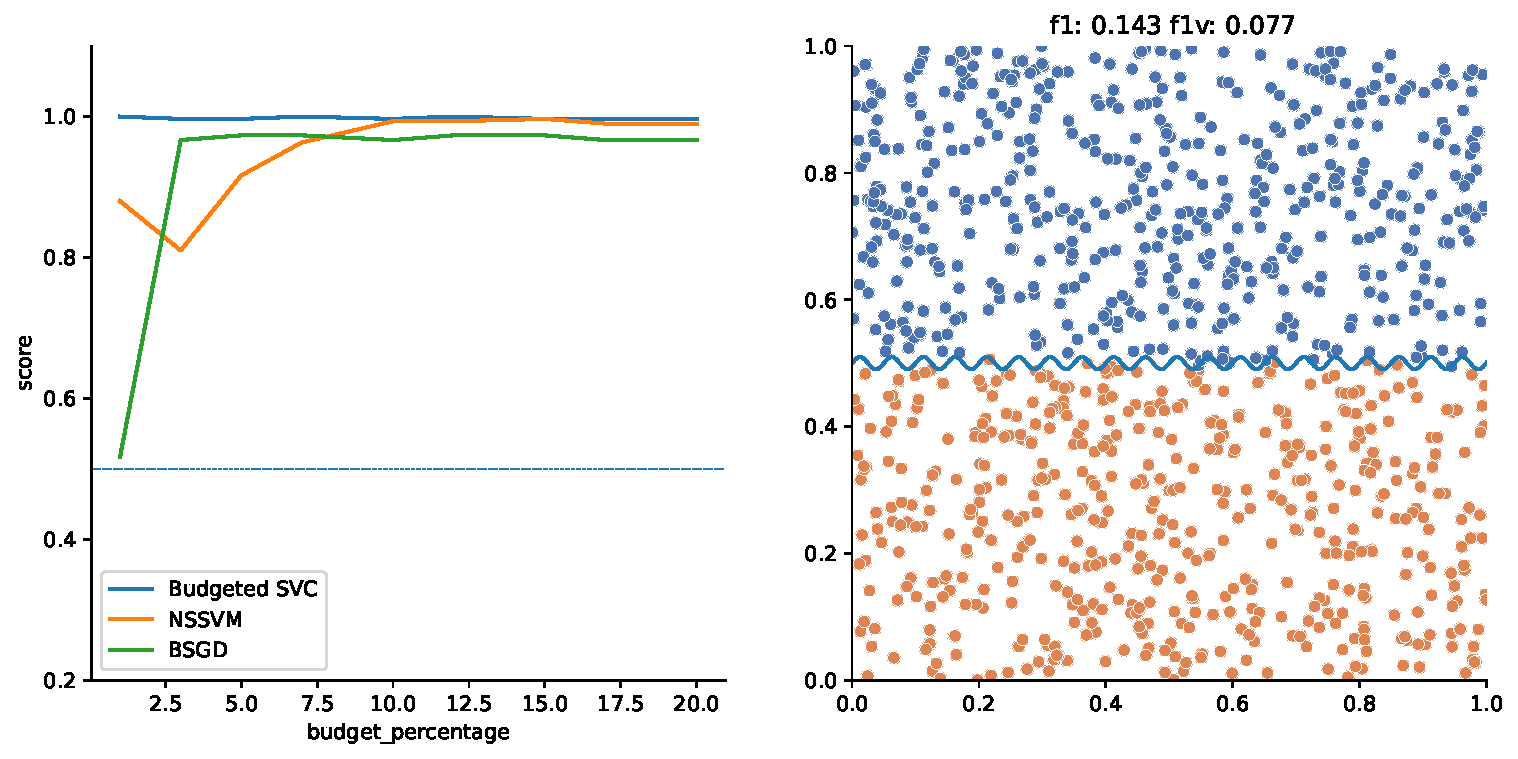
\includegraphics[width=\textwidth]{img/comp_new/6.pdf}
    \end{subfigure}%
    %
    \hfill
    %
    \begin{subfigure}{.5\textwidth}
        \centering
        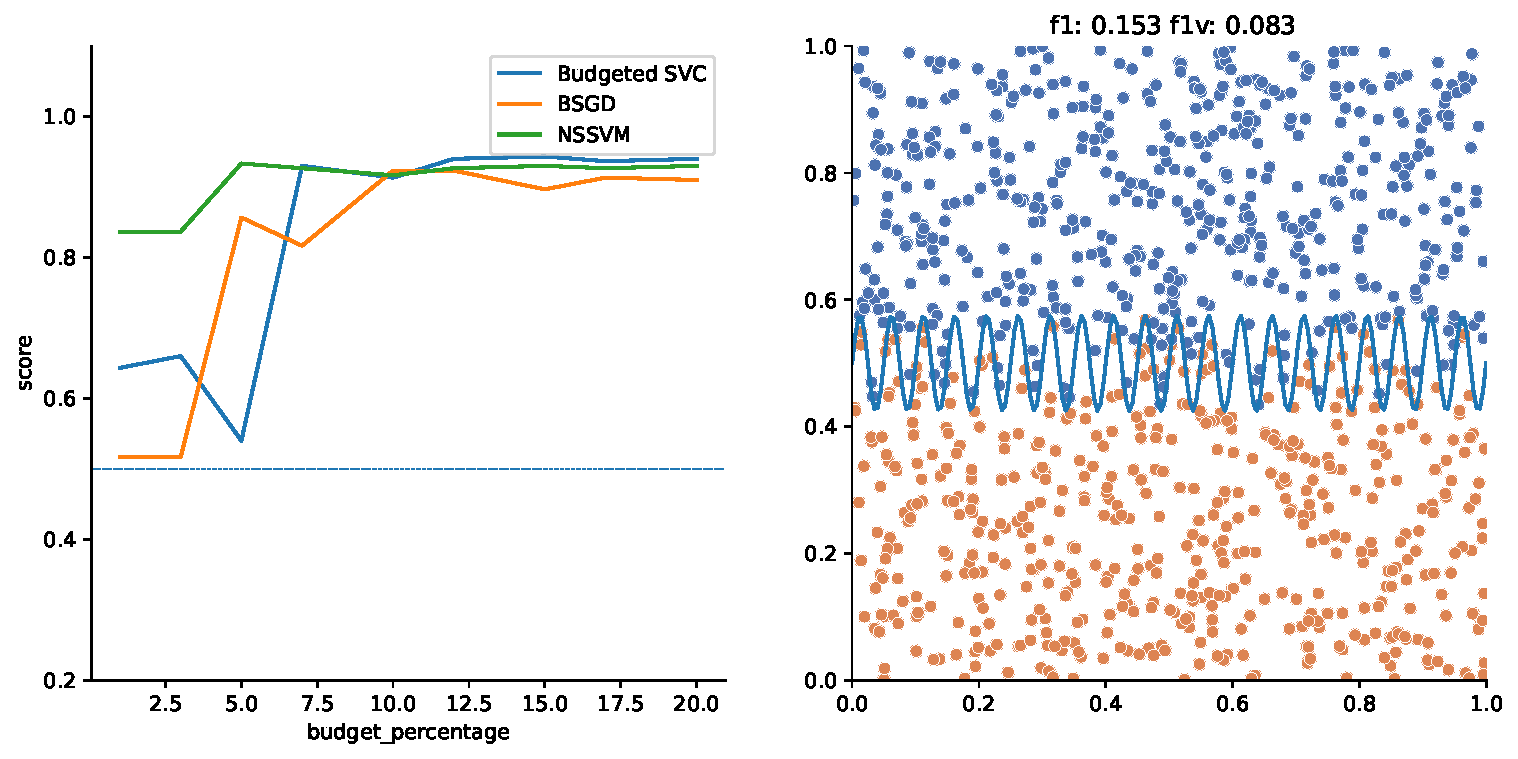
\includegraphics[width=\textwidth]{img/comp_new/9.pdf}
    \end{subfigure}
    \begin{subfigure}{.5\textwidth}
        \centering
        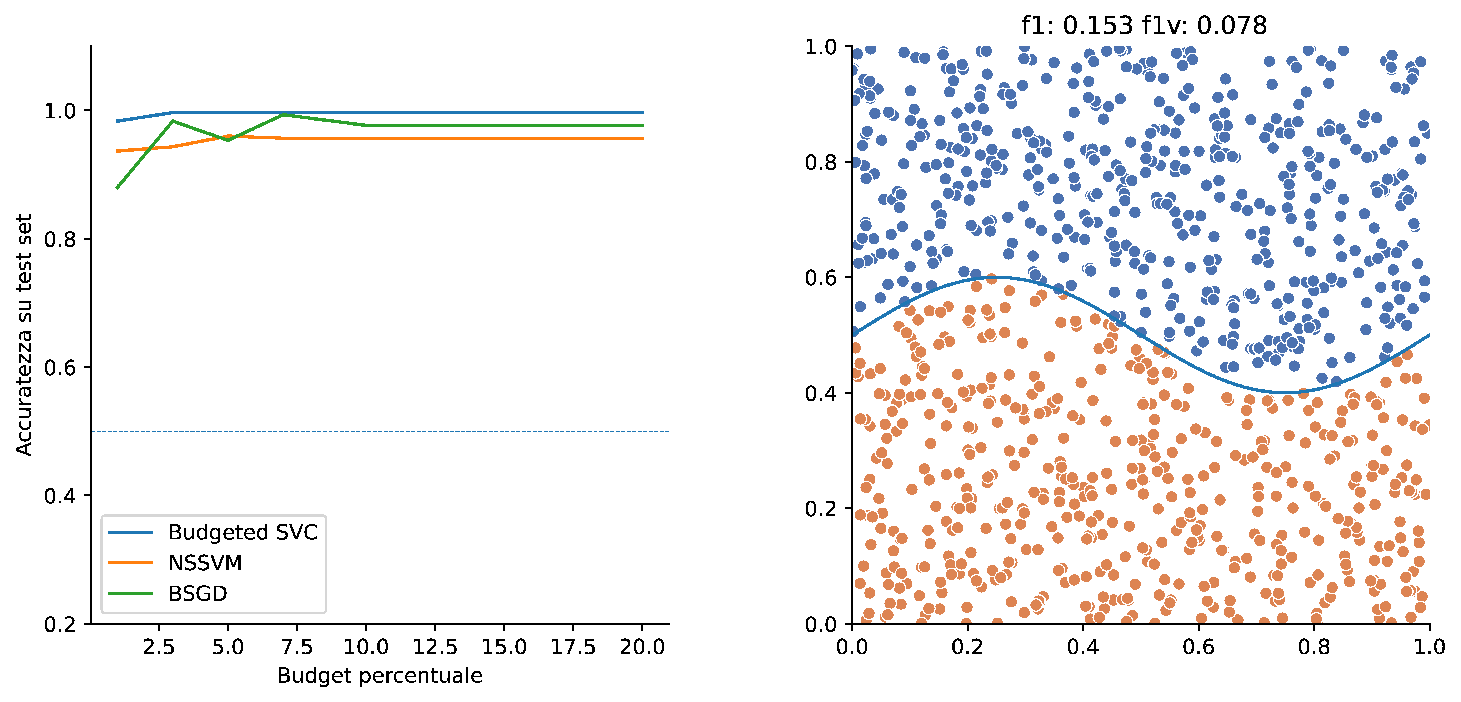
\includegraphics[width=\textwidth]{img/comp_new/10.pdf}
    \end{subfigure}%
    %
    \hfill
    %
    \begin{subfigure}{.5\textwidth}
        \centering
        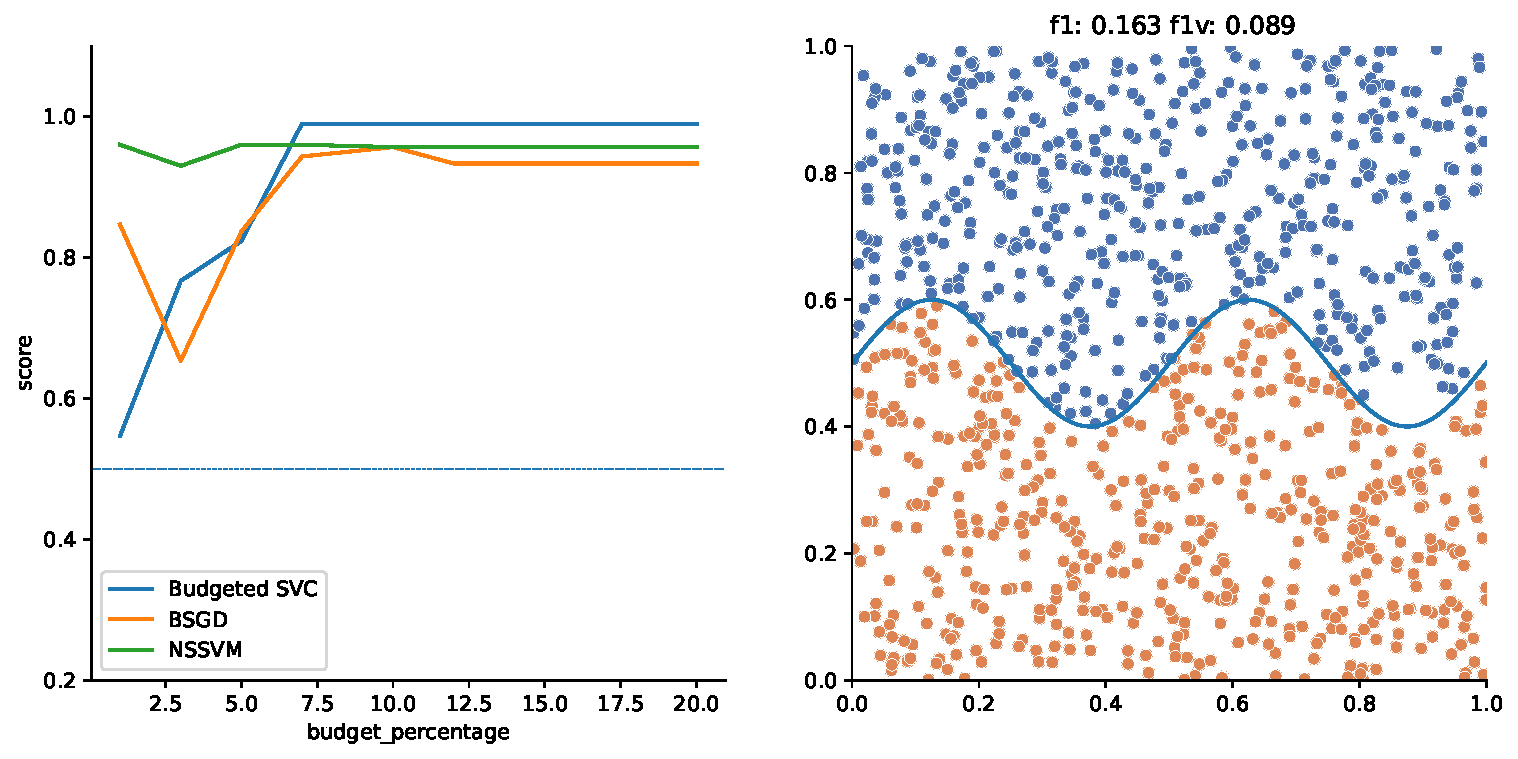
\includegraphics[width=\textwidth]{img/comp_new/11.pdf}
    \end{subfigure}
\caption{Questi grafici completano la~\Cref{fig:comp_new}.}
%\label{fig:comp_new}
\end{figure}


\end{appendices}